\begin{problem}{/images/problems/02_family_photos.jpg}{Ten photos}
	We have 10 photos with three people in each of them. In all photos, the person on the left is the father of the person in the middle and the person on the right is the uncle of the person in the middle. Also, all of the people on the left of the photos are distinct. What is the smallest number of people who are in the photos?\\[0.2cm]

	Link to the problem on Twitter:  \url{https://twitter.com/Riazi_Cafe/status/1663699752070905856}
\end{problem}

\begin{solution}.
	The correct answer is 16. \\[0.2cm]
	To prove this, we must first show that it is possible to make 10 photos with 16 people. Then we show that this is not possible with smaller than 16 people. Some people have already given a correct answer to the first part: see for example \url{https://twitter.com/AliAbdi_fa/status/1663881857862193153}.
	\begin{center}
		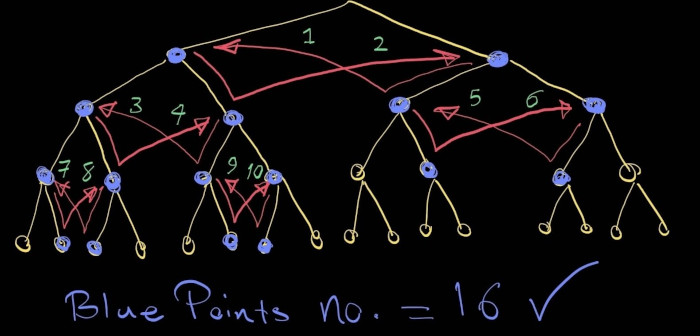
\includegraphics{/images/problems/02_diagram0.jpeg}
	\end{center}	
	Now we show why at least 16 distinct people have to be present in the photos. Let $a$ be the number of people who are neither a father in any photo nor an uncle in any photo (and thus they can only appear in the middle of each picture). Let $b$ be the number of people who are a father in at least one photo but not an uncles in any photo. Also let $c$ be the number of people who are an uncle in at least one photo but not a father an any photo. Finally, let $d$ be the number of people who are both an uncle in at least one photo and a father in at least one  photo. The total number of people in the photos is the sum of these 4 numbers. It can be proved that $a \geq d/2 + 1$ and because we have 10 photos with 20 uncles and fathers in them, $b + c + 2d = 20$. By putting the above inequalities together, we conclude $a + b + c + d \geq 21 - d/2$ and since we have 10 photos, $d$ is at most 10, so $a + b + c + d \geq 16$.\\[0.2cm]

	link to the solution on Twitter: \url{https://twitter.com/Riazi_Cafe/status/1664832603759824897}

\end{solution}